\documentclass[12pt]{article}
\usepackage[utf8]{inputenc}
\usepackage[T1]{fontenc}

\usepackage{graphicx}
\usepackage{authblk}
\graphicspath{ {img/} }

\begin{document}

\begin{titlepage}
  \centering
  {\scshape\LARGE HTL Wiener Neustadt \par}
  \vspace{1cm}
  {\scshape\Large NVS Project\par}
  \vspace{1.5cm}
  {\huge\bfseries Paint - sharing art is fun\par}
  \vspace{2cm}
  {\Large\itshape Nico Kratky\par}

  \vfill

  {\large \today\par}
\end{titlepage}

\section{Procedure}
Paint is a web application that allows connected useres to paint collaborativly. When the page is accessed the user is prompted to enter a username, which defaults to a random GUID (Globally Unique Identifier). If the user enters an invalid username, the whole process is repeated. After this, a random color is asigned to said user. This color can be changed via a command afterwards. Now the user is ready to draw. This can be done by clicking and dragging the left mouse button.


Under the drawing canvas there is a box which displays the current color, and a textbox that is used to enter commands.

\section{Commands}
\begin{itemize}

\item \textbf{\textit{/reset}} Alle Zeichnungen werden geloescht
\item \textbf{\textit{/color HEXCODE}} Die aktuelle Farbe wird auf \textit{HEXCODE} gesetzt
\item \textbf{\textit{/users}} Gibt eine Liste aller verbundenen Users aus

\end{itemize}

If the enterd text does not match a command, it is interpreted as a message and broadcasted to other connected clients.

\section{Division}
\paragraph{Nico Kratky}- Server
\paragraph{Nico Kratky}- Client

\pagebreak

\section{Protocol}
\begin{figure}[h]
    \centering
    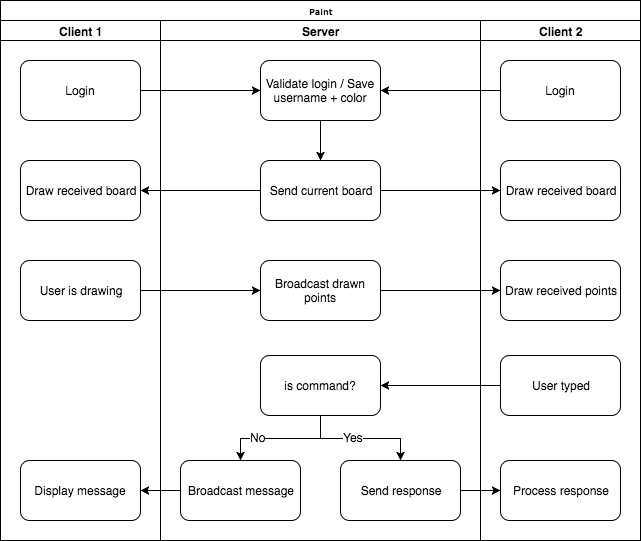
\includegraphics[width=0.7\textwidth]{protocol}
    \caption{Protocol used by paint}
    \label{fig:mesh1}
\end{figure}

\end{document}
